\section{User Interface Design}
  The mockups of the application were already presented in the RASD. This section illustrates the User Experience flow by using two User Experience diagrams. Both diagrams are pretty similar since some interfaces are the same for both common User and Authority. As we can see from the following diagrams the leftmost part is merely devoted to allow users to log into the application, and is composed by these elements:
\begin{itemize}
    \item Splash Screen
    \item Login
    \item Register
    \item Recovery Password
\end{itemize}

\vspace{4mm}
The Main Menu is different for User and Authority since an Authority is able to:
\begin{itemize}
\item View the violations notified by Users and generate traffic tickets
\item View the own traffic tickets generated
\item Get Suggestions
\end{itemize}
And the User is able to:
\begin{itemize}
\item Report a traffic violation
\item View the own reports list
\end{itemize}
However, both share also some other interfaces in addition to the ones related to the login:
\begin{itemize}
    \item Statistics
    \item Safe/Unsafe Areas
    \item Settings
    \item About SafeStreets
    \item Contact SafeStreets
\end{itemize}
\textit{Settings, About} and \textit{Contact SafeStreets} are accessible through the button in the top-left corner from the Main Menu. Those 3 activities were not shown on the mock-ups because aren't relevant for the Application functionality.

\begin{figure}[H]
\advance\leftskip-3cm
    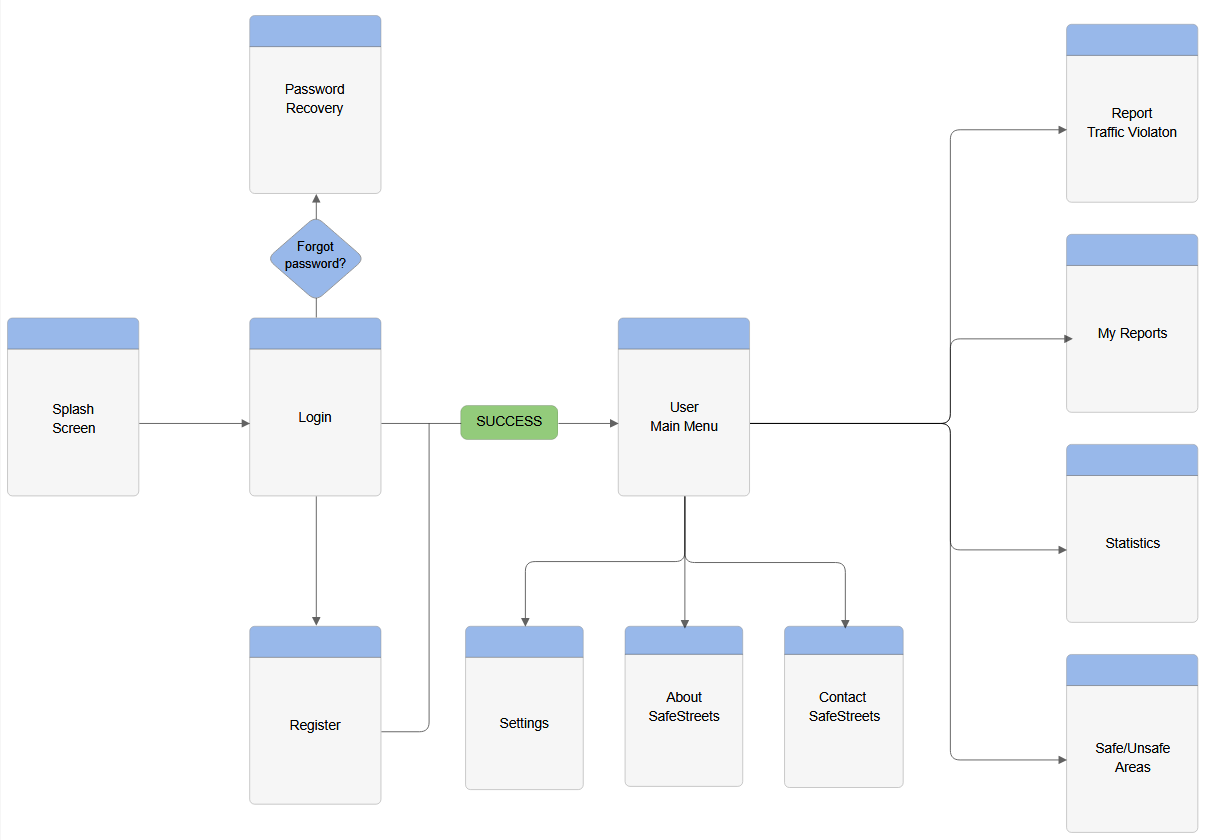
\includegraphics[width=1.5\textwidth,left]{Images/ux_user_definitivo.png}
    \caption{User UX Diagram}
\end{figure}
\begin{figure}[H]
\advance\leftskip-3cm
    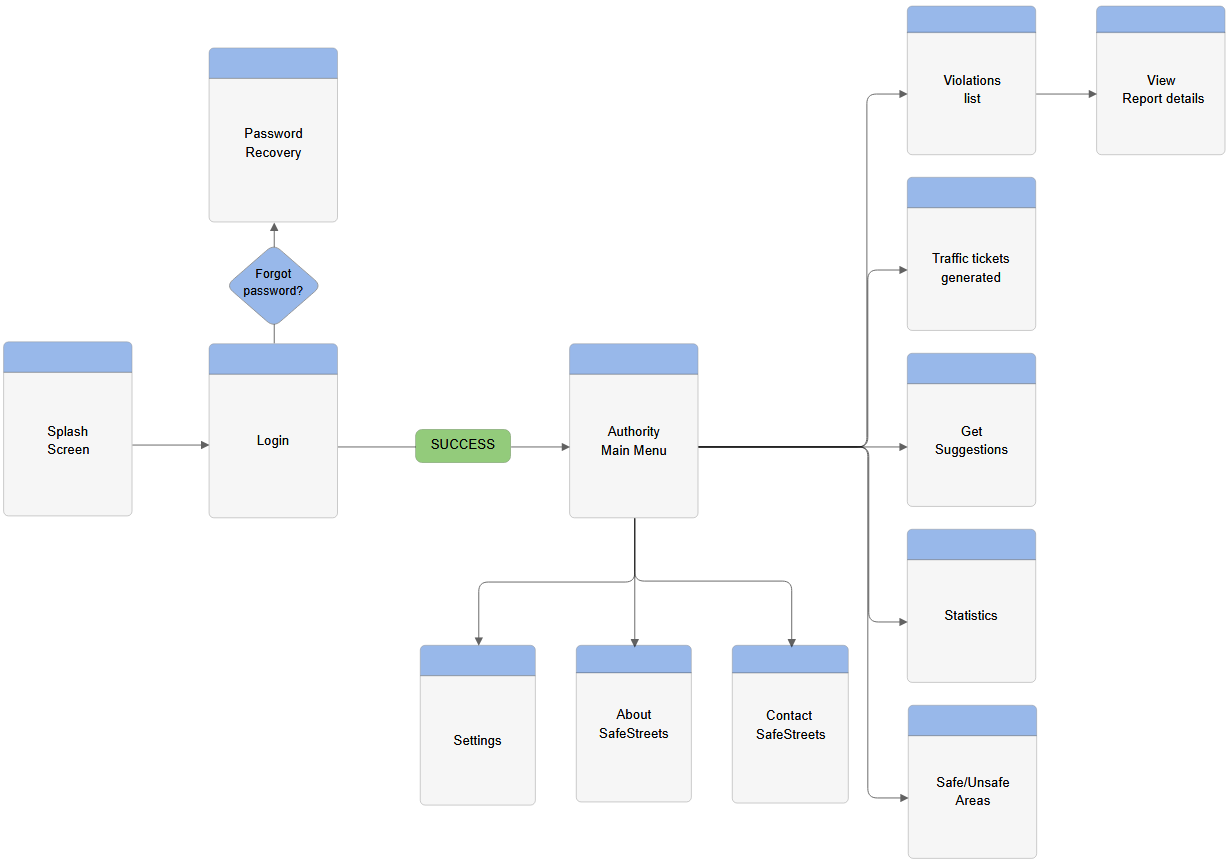
\includegraphics[width=1.5\textwidth,left]{Images/ux_authority_definitivo.png}
    \caption{Authority UX Diagram}
\end{figure}
\cleardoublepage